%\documentclass[10pt]{letter}
%\usepackage[utf8]{inputenc}

%%%%%%%%%%%%%%%%%%%%%%%%%%%%%%%%%%%%%%%%%%%%%%%%%
% compile with LuaLatex
%%%%%%%%%%%%%%%%%%%%%%%%%%%%%%%%%%%%%%%%%%%%%%%%%%%%%%%
\documentclass[11pt]{report}
\usepackage{epsfig}
\usepackage{amssymb,amsmath,amsfonts}
\usepackage[activeacute,american]{babel}
%\usepackage[utf8]{inputenc}
\usepackage{subfiles}
\usepackage{cite}
\usepackage{csquotes}
\usepackage{esvect}
\usepackage[acronym,nonumberlist]{glossaries}
\renewcommand{\acronymname}{Nomenclature}

\usepackage{caption} 
\usepackage{float}
\usepackage[
    math-style=ISO,      % Upper Case Greek is in italics
    bold-style=ISO,      % Bold math is in italics
    partial=upright,     % nabla and partial upright
    nabla=upright,
  ]{unicode-math}
\topmargin 1.2cm 
\textwidth 16.1cm
\textheight 22.5cm
\oddsidemargin 0.7cm
\setcounter{tocdepth}{5}
\addtolength{\voffset}{-2.4cm}
\addtolength{\hoffset}{-0.5cm}

\usepackage{setspace}
%\doublespacing
\onehalfspacing
\usepackage{caption}
 \captionsetup[figure]{labelfont={bf},name={Figura},labelsep=period}


%%%%%%%%%%%%%%%%%%%%%%%%%%%%%%%%%
\begin{document}
\centering{ \textbf{\Large{Mec\'anica de fluidos}}}

%\centering {\Large{2$^\circ$ semestre 2020: 541209-1}}
\vspace{1cm}

\flushleft{ \large \underline{\textbf{Pr\'actica 2: Fuerzas hidrost\'aticas sobre superficies y cuerpos sumergidos}}}

%%%%%%%%%%%%%%%%%%%%%%%%%
\vspace{1cm}

\underline {Problema 1 (P. 4.40 Mott\footnote{footnotes working fine}):}

\vspace{0.2cm}

La figura ~\ref{fig:fig1} muestra una compuerta rectangular que contiene agua tras ella. Si la profundidad del agua es de $6$ pies, calcule la magnitud y ubicaci\'on de la fuerta resultante sobre la compuerta. Adem\'as calcule la fuerza sobre la bisagra en la parte superior y sobre el tope en el fondo.

\begin{figure}[H]
\centering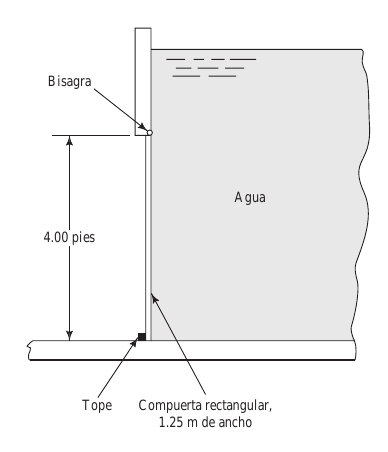
\includegraphics[width=0.5\textwidth]{p1.png}
\caption{\label{fig:fig1} }
\end{figure}

\footnotetext{Mott, Robert L. Mecanica de Fluidos 6/e. Pearson educación, 2006.}

%%%%%%%%%%%%%%%%%%%%%%%%%
\newpage
%%%%%%%%%%%%%%%%%%%%%%%%%

\underline {Problema 2 (P. 4.42 Fox):}

\vspace{0.2cm}

La figura ~\ref{fig:fig2} muestra un tanque de agua con un tubo circular conectado en su fondo. Una compuerta circular sella la abertura del tubo para impedir el flujo. Para drenar el tanque se utiliza una polea que abre la compuerta. Calcule la fuerza que debe ejercer el cable para abrir la compuerta.

\begin{figure}[H]
\centering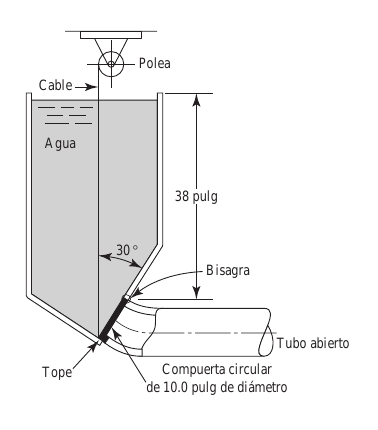
\includegraphics[width=0.5\textwidth]{p2.png}
\caption{\label{fig:fig2} }
\end{figure}

%%%%%%%%%%%%%%%%%%%%%%%%%
\vspace{0.5cm}
\underline {Problema 3 (P. 3.79 Fox):}
\vspace{0.2cm}

La figura~\ref{fig:fig3} esquematiza un cuerpo cil\'indrico de diametro $3$ m y largo $6$ m, el cual separa dos l\'iquidos. La gravedad espec\'ifica del l\'iquido a la izquierda es de 1.6 y la SG del l\'iquido de la derecha es de 0.8. Calcule la magnitud y direcci\'on de la fuerza resultante sobre el cilindro.

\begin{figure}[H]
\centering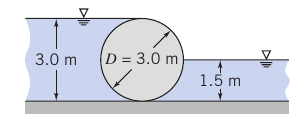
\includegraphics[width=0.5\textwidth]{p3.png}
\caption{\label{fig:fig3} }
\end{figure}

\footnotetext{Pritchard, Philip J. Fox and McDonald’s Introduction to Fluid Mechanics (8th ed.). John Wiley $\&$ Sons. (2011).}

%%%%%%%%%%%%%%%%%%%%%%%%%
\newpage
%%%%%%%%%%%%%%%%%%%%%%%%%

\vspace{0.5cm}
\underline {Problema 4 (P. 2.93 Munson\footnote{footnotes working fine}):}
\vspace{0.2cm}

El estanque cerrado presentado en la figura ~\ref{fig:fig4}, posee un domo semi-esf\'erico de diametro $4$ ft en su superficie superior. El estanque se encuentra lleno de agua. Adem\'as, al estanque se conecta un manometro diferencial de tubo en U. Determine la fuerza neta que se ejerce sobre el domo, considerando que la lectura del manometro diferencial es de $7$ ft y que la presi\'on del aire al final superior del manometro es de 12.6 psi (man\'ometricos).

\begin{figure}[H]
\centering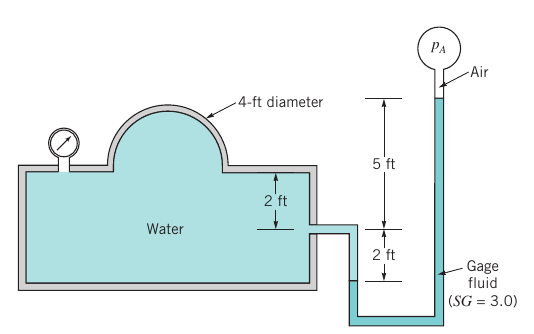
\includegraphics[width=0.5\textwidth]{p4.png}
\caption{\label{fig:fig4} }
\end{figure}

\footnotetext{Munson, Bruce R., et al. "Fundamentals of Fluid Mechanics, John Wiley $\&$ Sons." Inc., USA (2006).}

%%%%%%%%%%%%%%%%%%%%%%%%%
%%%%%%%%%%%%%%%%%%%%%%%%%


\vspace{0.5cm}
\underline {Problema 5 (P. 3.109 Fox):}
\vspace{0.2cm}

Un bowl es invertido simetricamente y se sumerge en un fluido denso (SG=15.6) a una profundidad de $200$ mm, medidos desde la superficie libre hasta el borde del bowl (figura~\ref{fig:fig5}). La altura del bowl es de $80$ mm y el fluido sube $20$ mm dentro del bowl. El bowl tiene un diametro interior de 100 mm y esta hecho de una arcilla cuya gravedad espec\'ifica es de 6.1. El volumen del bowl en s\'i es de 0.9 L. Calcule la fuerza requerida para mantener el bowl en equilibrio. 

\begin{figure}[H]
\centering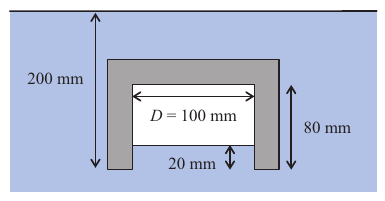
\includegraphics[width=0.5\textwidth]{p5.png}
\caption{\label{fig:fig5} }
\end{figure}

%%%%%%%%%%%%%%%%%%%%%%%%%
\newpage
%%%%%%%%%%%%%%%%%%%%%%%%%

\vspace{0.5cm}
\underline {Problema 6 (P. 3.89 Fox):}
\vspace{0.2cm}

Un hidr\'ometro es un instrumento que permite medir la gravedad espec\'ifica de un fluido. El valor medido por este instrumento ser\'a indicado por el nivel en el que la superficie libre intersecta el tallo vertical del equipo cuando este se encuentra flotando en el l\'iquido. La marca que indica $1.0$ corresponde al nivel para el hidr\'ometro flotando en agua destilada. Para el equipo presentado en la figura~\ref{fig:fig6}, el volumen sumergido para agua destilada es de $15$ cm$^3$. El tallo del hidr\'ometro tiene $6$ mm de diametro. Calcule la distancia $h$, desde la marca $1.0$ a la superficie del fluido, cuando el hidr\'ometro flota en acido n\'itrico, cuyo peso espec\'ifico es de $1.5$.

\begin{figure}[H]
\centering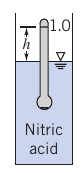
\includegraphics[width=0.2\textwidth]{p6.png}
\caption{\label{fig:fig6} }
\end{figure}

%%%%%%%%%%%%%%%%%%%%%%%%%
\end{document}
